\chapter{Migration Jira/Java Correction WorkBench}

\section{Qu'est-ce que Jira et Java Correction WorkBench}
Jira\index{Jira} est un loigiciel de tra\c{c}abilit\'{e} des probl\`{e}mes d\'{e}velopper par Atlassian dont l'usage est gratuit pour les organisations \`{a} but non lucratif, de charit\'{e} ou les projet open-source. SAP désire migrer de système de traçabilité pour utiliser maintenant Java Correction WorkBench\index{Java Correction WorkBench} (JCWB ou CWB).\\

JCWB est un logiciel............. voir Fabien



\section{Pr\'{e}sentation du contexte}

Comment cela se passe actuellement \`{a} SAP
à SAP tous les codes des différents projets sont hébergés sur le gestionnaire de version Perforce\index{Perforce} (SCM : Source Code Management)
et ceux-ci sont compilés plusieurs fois chaque jour grâce à Jenkins\index{Jenkins} ou ASTEC (CIS : Continuous Integration Software).\\
Chaque projet se compose d'une part son code source mais aussi d'une grande quantité de tests qui sont joués pour garantir\footnote{La valeur de la garantie dépends directement du test coverage} le bon fonctionnement du produit. Lorsqu'il y a un problème sur la build, que ce soit une erreur de compilation ou un test qui échoue, le statuts de la build change en fonction du problème. Dès lors que quelqu'un c'est aperçu du problème celui-ci inscrit un defect\index{Defect} dans Jira\footnote{L'utilité de Jira est bien plus large que la simple déclaration d'un test échoué, il sert à décrire n'importe quel problème quelle que soit la version, la branche ou le produit}.\\


\subsection{Plugin de reporting}
Pour leur permettre d'avoir un rapport visuel sur l'état des builds, ils utilisent le plugin Radiator. Ce plugin permet l'affichage, sur un seul écran divisé, des groupes de jobs\footnote{Typiquement, un job correspond à un projet logiciel}. Un groupe de jobs est un carré coloré dont la couleur représente l'état des jobs qui le compose.\\
Les statuts pris en compte sont les statuts Jenkins\footnote{Error, Failure, Unstable, Aborted, Not built, Success} ainsi qu'un statuts supplémentaire issue du plugin Claim. Ce plugin permet à un développeur de claim une erreur, c'est-à-dire que le projet comporte une imformation supplémentaire qui est un nom d'utilisateur et le message que celui-ci a laisser.


En résumé Radiator :
\begin{itemize}
	\item permet de rassembler les jobs en un seul groupe de jobs
	\item où chacun des jobs a un statuts\footnote{statuts Jenkins}
	\item le groupe de projet arborant la couleur jugée la plus importante
	\item de prendre en compte les informations supplémentaires du plugin claim
\end{itemize}
Par exemple, si nous avons deux groupes composés chacun de trois jobs, tous différents. Supposons que, sur les 6 jobs, l'un soit en échec les autres étant en succès. Nous aurons donc une vue colorée en verte (parce que tous les projets sont en succès) et la deuxième vue apparaissant en rouge (l'un des jobs ayant échoués) ou bien en orange si l'échec est investigué (échec claim par un développeur).\\




\textbf{Problème}\hfill \\ \indent
Cette solution permet de visualiser les statuts des jobs mais ne fait pas de distinction parmis les jobs échoués. Parmis ceux-ci on peut distinguer :

\begin{itemize}
	\item les jobs échoués depuis très longtemps
	%%\item les jobs échoués en cours d'investigation
	\item les jobs échoués avec un defect\index{Defect} enregistré
\end{itemize}
L'inconvénient est que les tests échoués récemment et non reconnus apparaissent de la même manière que les tests échoués et reconnus. La solution provisoire mais permettant de ne plus polluer l'affichage avec du rouge, conciste à faire passer les jobs en échecs avec defect\index{Defect} (ie. reconnus et enregistrés comme échecs dans Jira\index{Jira} ou CWB\index{Java Correction WorkBench}) sont passés en vert.\\
De cette manière, seul les nouveaux échecs apparaissent en rouge. En grande partie des régressions.\\
Le revers de la médaille est que l'affichage n'est plus représentatif de la réalité, une partie de l'information est perdue puisqu'un test apparaissant en succès peut en fait ne pas l'être.\\




Sauf qu'actuellement seuls les defects rentrés sur Jira sont pris en compte, la mécanique en place ne permet pas encore de récupérer ces mêmes informations de CWB\index{Java Correction WorkBench}. \\
Puisque de plus en plus de defects seront enregistrés sur CWB, et dans un soucis d'homogénéisation du process actuel, il faut rationnaliser le process actuel et permettre au statuts d'être ajustés quelque soit l'origine du defect (Jira ou CWB).\\




\section{Process actuel}

1- Investigation du process actuel

la méthode apply de JUnit est surchargée\\
il y a une annotation qui permet de checker le status\\
l'annotation est prise en compte en fonction d'un paramètre -D\\

même résultat pour acceptance et GTP ????   ->> fabien\\

Dans l'état actuel des choses le process utilisé est illustré figure \ref{figure:bugManagementProcess} page \pageref{figure:bugManagementProcess}

\begin{figure}[!h]
  \centering
      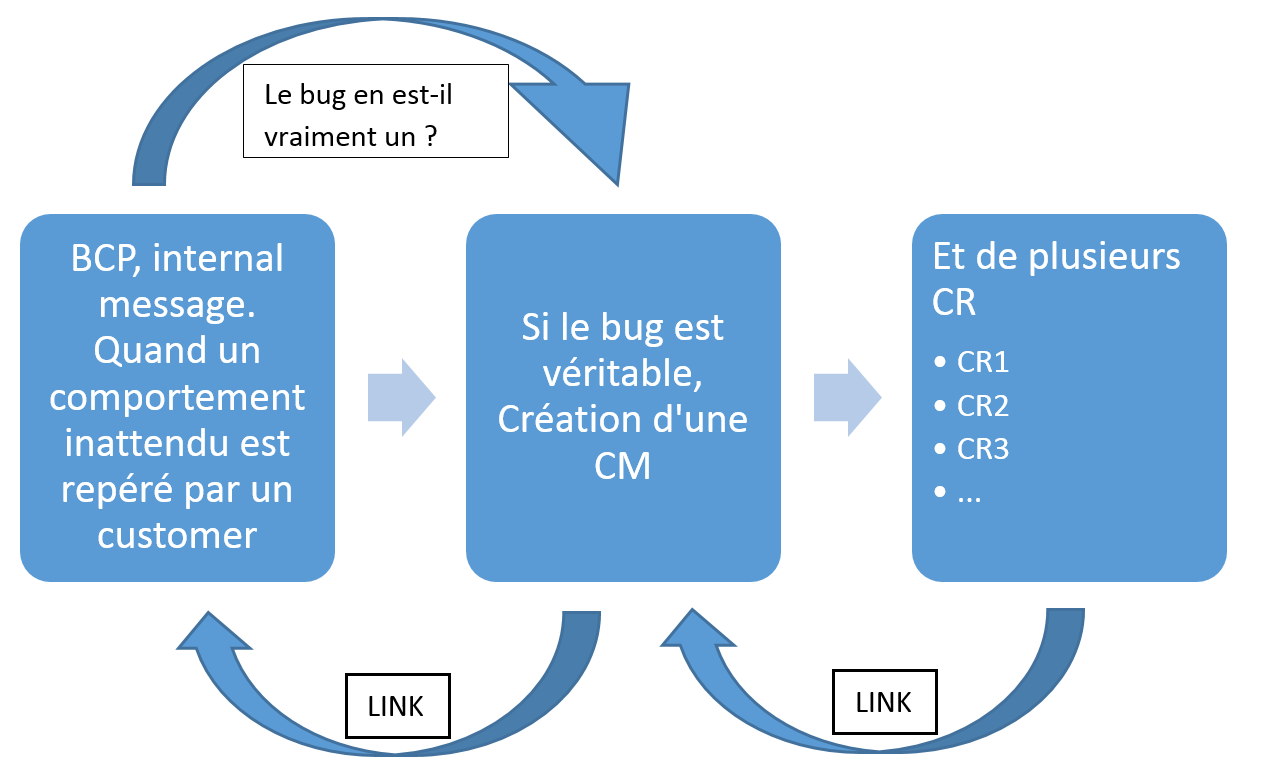
\includegraphics[width=\textwidth]{images/bugManagementProcess.png}
  \caption{Le process utilisé lors de gestion d'un bug}
	\label{figure:bugManagementProcess}
\end{figure}





\textbf{En résumé}\hfill \\ \indent 
\begin{itemize}
	\item JUnit est surchargé par la classe JiraIssueWatcher.java
	\item Je vais devoir utiliser le système choisi par SAP pour fournir les credentials : \Large{prod-pass-access}\normalsize
	\item Il existe une API permettant d'obtenir les informations que je désire : \Large{CWB HTTP API}\normalsize
\end{itemize}




\section{Travail effectué}


La première partie du travail s'est cantonée à des recherches et des échange de mails internes à SAP.\\

!!!!!  Ici je décris mes différents mails avec marco et Fabien!!!!!\\


\subsection{Fonctionnement et utilisation de prod-pass-access}






